\section{Apprendimento Bayesano}
Nell'ambito Bayesano si cambia l'approccio avendo la valutazione di ipotesi in base alla loro probabilità. Si studia la probabilità rispetto ai dati e rispetto
alle conoscenze pregresse. Non troviamo un'ipotesi che combacia ma che è probabile.\\

Bisogna studiare come scegliere le ipotesi, usando risultati noti del calcolo probabilistico e quindi come funziona l'apprendimento. Useremo le nozioni di probabilità e probabilità condizionata, oltre ovviamente alla \textbf{regola di Bayes}. Il meglio è definito quindi tramite probabilità.\\ 

Si assume quindi che le quantità di interesse siano governate da distribuzioni di probabilità e che la decisione migliore può essere presa ragionando su tali distribuzioni e sull'insieme di dati di training. L'apprendimento Bayesano è importante per due ragioni principali: 
\begin{enumerate}
  \item si ha una manipolazione esplicita delle probabilità rispetto ad altri approcci pratici di alcuni tipi di problemi di apprendimento (infatti si hanno spesso paragoni con gli alberi decisionali e con le reti neurali)
  \item fornisce una prospettiva utile per comprendere metodi di apprendimento che non manipolano effettivamente le probabilità
\end{enumerate}

Andando a considerare quelle che sono le caratteristiche del Bayesiano, si ha che ogni esempio di training osservato può aumentare o diminuire, in modo incrementale, la stima di probabilità relativa alla correttezza di un'ipotesi. Inoltre, come già anticipato, la conoscenza pregressa può essere combinata con i dati osservati per determinare la probabilità finale delle varie ipotesi. \\

Si ha inoltre che le varie ipotesi possono effettuare predizioni probabilistiche, le nuove istanze possono essere classificate combinando le predizioni delle ipotesi, che sono pesate attraverso la loro stessa probabilità. Con il metodo Bayesano si ottiene quindi uno standard per prendere decisioni ottimali attraverso il quale, altre misure pratiche, possono essere misurate. \\

Si hanno però alcune difficoltà legate all'apprendimento Bayesano:
\begin{itemize}
  \item si necessita avere la conoscenza di varie probabilità
  \item si hanno costi computazionali non indifferenti
\end{itemize}

\subsection{Teorema di Bayes}
Ponendo l'attenzione nel macchine learning dove si è interessati a trovare la migliore ipotesi $h$, presente in uno spazio delle ipotesi $H$, una volta eseguito l'addestramento su un training data $D$.  Il teormea di Bayes(o se vogliamo nell'apprendimento Bayesano) si ragiona in termini differenti, si ha che la miglior ipotesi altro non è che la più probabile. Per quanto riguarda la probabilità, la possiamo calcolare basandoci: sulla probabilità conosciuta a priori, sulla distribuzione dei dati che vado a osservare o dai dati stessi. 

\begin{teorema}{Teorema di Bayes}{}
    Il teorema enuncia che: \[P(h|D)=\frac{P(D|h)P(h)}{P(D)}\]
    Avendo:
    \begin{itemize}
        \item $P(h)$:   probabilità conosciuta a priori di $h$. Tale probabilità riflette qualsiasi conoscenza di base sulla possibilità che $h$ sia corretta  
        \item $P(D)$:   probabilità conosciuta a priori di $D$, ovvero la probabilità che $D$ sia osservato
        \item $P(D|h)$: probabilità di osservare $D$ in presenza dell'ipotesi $h$
        \item $P(h|D)$: probabilità a posteriori di $h$. Tale probabilità riflette la confidenza che $h$ sia valida dopo che $D$ è stato osservato
    \end{itemize}
\end{teorema}

Cercando di semplificare l'approccio computazione, evitando quindi di considerare tutte le $D$ e tutte le $h$, esistono altre soluzioni. 
In molti scenari di apprendimento, il learner considera un insieme di ipotesi candidate $H$ ed è interessato a trovare l'ipotesi più probabile $h\in H$, in base ai dati osservati in $D$.\\
Definiamo le ipotesi \textit{ maximum a posteriori (MAP)} ogni ipotesi massimamente probabile e la indichiamo:
    \begin{equation*}
        \begin{split}
            h_{MAP}&=\operatorname*{argmax}_{h\in H}P(h|D)\\
            & = \operatorname*{argmax}_{h\in H}\frac{P(D|h)P(h)}{P(D)}\\
            & = \operatorname*{argmax}_{h\in H}P(D|h)P(h)
        \end{split}
    \end{equation*}
L'ultimo passaggio viene eseguendo tenendo nota che $P(D)$ può essere cancellato in quanto costante e indipendente da $h$.\\

Spesso si assume anche che ogni ipotesi è a priori equiprobabile e quindi possiamo semplificare ulteriormente i conti. Dato che $P(D|h)$ viene spesso chiamata \textbf{likehood (\textit{probabilità})} di $D$ data $h$ viene definita ipotesi\textbf{ maximum likehood (ML)} ogni ipotesi che massimizza $P(D|h)$ descrita come segue: \[h_{ML}=\operatorname*{argmax}_{h\in H}P(D|h)\]
potendo quindi trascurare $P(h)$ in quanto costante e uguale $\forall\,h\in H$\\

Si può usare il teorema di Bayes per specificare un algoritmo di apprendimento molto semplice detto \textbf{algoritmo Brute-Force MAP LEARNING} che si articola
in 2 step:
\begin{enumerate}
  \item $\forall\,h\in H$ calcolo la probabilità a posteriori tramite il teorema di Bayes: \[P(h|D)=\frac{P(D|h)P(h)}{P(D)}\]
  \item restituisco l'ipotesi $h_{MAP}$ con la più alta probabilità a posteriori: \[h_{MAP}=\operatorname*{argmax}_{h\in H}P(h|D)\]
\end{enumerate}
Per specificare un problema di apprendimento per l'algoritmo bisogna specificare i valori di $P(h)$ e $P(D|h)$, e in base a questo dobbiamo fare alcune assunzioni:
\begin{itemize}
  \item il training set deve essere privo di rumore, avendo: $d_i=c(x_i)$
  \item il target concept deve essere contenuto nello spazio delle ipotesi $H$, dettagliatamente si dirò che: 
  $\exists h\in H \ : \  \forall\, x\in X$ si ottiene che $ h(x)=c(x)$
  \item devo assumere che le ipotesi siano equiprobabili e quindi: $P(h)=\displaystyle \frac{1}{|H|}\quad \forall h\in H$
  riducendoci ad avere:
  \[P(D|h)=
    \begin{cases}
      1&\mbox{se } d_i=h(x_ i),\,\,\,\forall\,d_i\in D\\
      0&\mbox{altrimenti}
    \end{cases}
  \]
\end{itemize}

Ora che abbiamo completamente definito l'algoritmo di apprendimento, in un primo passaggio dobbiamo determinare le probabilità dei nostri $P(h|D)$:
\begin{itemize}
   \item $h$ è inconsistente con $D$, avendo quindi: $P(h|D)=\displaystyle\frac{0\cdot P(h)}{P(D)}=0$
  \item $h$ è consistente con $D$, avendo quindi: $\displaystyle P(h|D)=\frac{1\cdot \frac{1}{|H|}}{P(D)} = \frac{1\cdot \frac{1}{|H|}}{\frac{|V\ S_{H,D}|}{|H|}}=\frac{1}{|V\ S_{H,D}|}$ 
\end{itemize}
Questa analisi implica il fatto che, in base a queste assunzioni, ogni iptotesi consistente è una ipotesi $MAP$, questo perché $\forall h$ che è consistente, $\displaystyle P(h|D) = \frac{1}{|V\ S_{H,D}|}$

\begin{figure}[H]
    \centering
    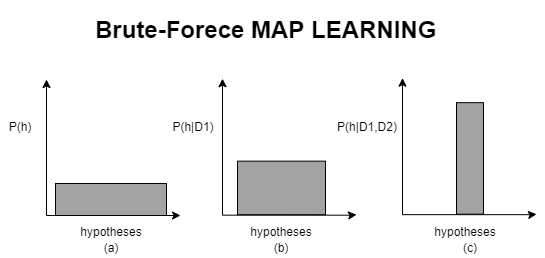
\includegraphics[scale = 0.7]{imm/foto_map.png}
\end{figure}
Dove (a) corrisponde a dire che tute le ipotesi hanno la stessa probabilità, invece (b)+(c) si ha che mentre i dati di addestramento si accumulano, la probabilità a posteriori delle ipotesi inconsistenti diventa zero mentre la probabilità totale che si somma a 1 è condivisa in maniera equa tra le ipotesi consistenti rimanenti.\\

Si ha che ogni learner consistente ha in output ipotesi MAP, se si assume a priori la distribuzione uniforme delle probabilità su $H$ dati di training deterministici e privi di rumore.\\

Riprendendo l'algoritmo find-S si ha che: 
\begin{itemize} 
    \item ha in output ipotesi consistenti e quindi ipotesi MAP sotto la distribuzione di probabilità $P(h)$ e $P(D|h)$ 
    \item $\forall\,P(h)$ che favorisce le ipotesi più specifiche, find-S trova appunto le ipotesi MAP 
\end{itemize} 

A riprova che il metodo Bayesano è un modo per caratterizzare il comportamento degli algoritmi di apprendimento, identificando le distribuzione di probabilità $P(h)$ e $P(D|h)$ in base alle quali l'output è l'ipotesi ottimale, è possibile caratterizzare le ipotesi implicite dell'algoritmo ovvero il \textbf{bias induttivo}.\\

Si introduce ora il problema di apprendere funzioni target a valori continui (coime reti neurali o regressione lineare). Si ha che in base a determinate assunzioni, qualsiasi algoritmo di apprendimento che minimizzi l'errore quadratico (scarto quadratico??) tra l'ipotesi di output e i dati di addestramento, produrrà un'ipotesi ML.\\
Si imposta il problema come segue:
\begin{itemize}
    \item $\forall\,h\in H$,  $h:X\to\Re$, avendo esempi della forma $\langle x_i, d_i\rangle$
    \item la funzione target è definita come $f:X\to\Re$
    \item si hanno $m$ esempi di training dove il valore target di ogni esempio è sporcato dal rumore casuale secondo una distribuzione di probabilità normale con media nulla, avendo $d_i=f(x_i)+e_i$
\end{itemize}

Avendo quindi che $h_{ML}=\operatorname*{argmax}_{h\in H}P(D|h)$ e che gli eventi di training vengono assunti come indipendenti si ha che: $$h_{ML}=\operatorname*{argmax}_{h\in H}\prod_{i=1}^mP(d_i|h)$$ \\

Dato quindi l'errore ($e_i$) distribuito normalmente con media zero e varianza sconosciuta $\sigma^2$ si ha che anche ogni $d_i$ deve seguire la stessa distribuzione attorno al valore target $f(x_i)$. Poiché stiamo scrivendo l'espressione per $P(D|h)$, assumiamo che $h$ sia la descrizione corretta per $f$, quindi: $\mu=f(x_i)=h(x_i)$, e avendo quindi, per la distribuzione normale: 
\[h_{ML}=\operatorname*{argmax}_{h\in H} \prod_{i=1}^m\frac{1}{\sqrt{2\pi\sigma^2}} e^{-\frac{1}{2\sigma^2}(d_i-h(x_i))^2}\]
È comune massimizzare il logaritmo meno complicato, il che è ragionevole per via della monotonia di questa funzione, ottenendo:
\[h_{ML}=\operatorname*{argmax}_{h\in H}\sum_{i=1}^m\ln{\frac{1}{\sqrt{2\pi\sigma^2}}} -\frac{1}{2\sigma^2}(d_i-h(x_i))^2\]
ma il primo termine è costante e indipendente da $h$ e quindi può non essere considerato:
\[h_{ML}=\operatorname*{argmax}_{h\in H}\sum_{i=1}^m -\frac{1}{2\sigma^2}(d_i-h(x_i))^2\]
Sapendo che massimizzare questo termine negativo equivale a ridurre al minimo il termine positivo corrispondente:
\[h_{ML}=\operatorname*{argmin}_{h\in H}\sum_{i=1}^m \frac{1}{2\sigma^2}(d_i-h(x_i))^2\]
e avendo che anche tutte le costanti sono indipendenti da $h$ e quindi possono essere rimosse:
\[h_{ML}=\operatorname*{argmin}_{h\in H}\sum_{i=1}^m (d_i-h(x_i))^2\]
trovando che $h_{ML}$ è ciò che minimizza gli errori quadratici. \\

Si specifica la scelta della normale in quanto:
\begin{itemize}
  \item buona approssimazione di molti tipi di rumore nei sistemi fisici 
  \item il Teorema del Limite Centrale mostra che la somma di un numero sufficientemente grande di variabili casuali indipendenti e identicamente distribuite obbedisce a una distribuzione Normale
\end{itemize}

Si considera solo il rumore sul valore del target e non sugli attributi che descrivono le istanze stesse.\\ 
Anche in questo caso si usa il Rasoio di Occam, scegliendo di usare il principio \textbf{Minimum Description Length (\textit{MDL})}, scegliendo la spiegazione più breve per i dati osservati.\\

%% qui dice che riprenderà una slide

\subsection{Classificatore Bayesano ottimale per la classificazione}
Ci si chiede quindi qual è la classificazione più probabile della nuova istanza secondo i dati di training.\\
Applicare solamente $h_{MAP}$ non basta, questo perché non risulta la migliore situazione in alcune situazioni. \\

%%%Solo xk poi lo usa come concetto:
Sia $H = \{h_1,h_2,h_3\}$, dove $P(h_1)=  0.4$, $P(h_2) = P(h_3) =  0.3$, e sia $h_{MAP} = h_1$. Diciamo che $h_{MAP} = h_1$ semplicemente perché, tra i valori corrispondenti di probabilità, quella di $h_1$  è la più grande tra tutte ( $0.4 > 0.3$ )\\
Un diverso approccio ci porterebbe a una valutazione dell'istanza $x$ tale che questa venga classificata positiva grazie all'ipotesi $h_1$, ma negativa con le ipotesi $h_2, h_3$.\\
Avessimo valutato la probabilità in una maniera differente ci saremmo accorti che la probabilità che $x$ sia positiva è $0.4$,e che sia negativa pari a $0.6$.
E si nota facilmente che la classificazione più probabile non è quella di $h_{MAP}$.

Abbiamo che la classificazione più probabile si ottiene combinando le previsioni di tutte le ipotesi, ponderate in base alle loro probabilità posteriori.
 \[P(v_j|D)=\sum_{h_i\in H}P(v_j|h_i)P(h_i|D)\]
Dove $P(v_j|D)$ è la probabilità che la classificazione corretta sia $v_j$. Da questo possiamo ottenere il classificatore Bayesano ottimo 
\[\operatorname*{argmax}_{v_j\in V}\sum_{h_i\in H}P(v_j|h_i)P(h_i|D)\] Dove $V$ corrisponde alle etichette disponibili per il mio problema. 

\subsection{Classificatore Bayesano naive}
Il Classificatore Bayesano naive si applica alle attività di learning in cui ogni istanza $x$ è descritta da una giunzione di valori di attributi e in cui la funzione target $f(x)$ può prendere qualsiasi valore dall'insieme finito $V$ come parametro. Descriviamo gli esempi di training come $\langle a_1, a_2,\ldots a_n\rangle $. \\
Applicando il metodo Bayesano si ha:
\begin{equation*}
    \begin{split}
        v_{MAP}&=\operatorname*{argmax}_{v_j\in V}P(v_j|a_1, a_2,\ldots a_n)\\
        & =\operatorname*{argmax}_{v_j\in V}\frac{P(a_1, a_2,\ldots a_n|v_j)P(v_j)}{P(a_1, a_2,\ldots a_n)}\\
        & =\operatorname*{argmax}_{v_j\in V}P(a_1, a_2,\ldots a_n|v_j)P(v_j)
    \end{split}
\end{equation*}
Avendo che:
\begin{itemize}
    \item $P(v_j)$ può essere stimato tramite la frequenza di $v_j$ in $D$
    \item $P(a_1, a_2,\ldots a_n|v_j)$ non può essere stimato in questo modo, in questo caso il numero di termini è pari a $|X|\cdot |V|$
\end{itemize}
Con il classificatore Bayesano naive si hanno diverse semplificazioni. I valori degli attributi sono condizionatamente indipendenti significa che $P(a_1, a_2,\ldots a_n|v_J)=\prod_iP(a_i|v_j)$. E che a sua volta il numero dei termini $a_1, a_2,\ldots a_n$ è pari a: \[|\textnormal{Attributi distinti}|\cdot |\textnormal{Valori target distinti}|+|\textnormal{Valori target distinti}|\]
Non si ha quindi la ricerca esplicita all'interno del insieme delle ipotesi $H$, ma viene eseguito solo il conto delle frequenze.
Si ha quindi il classificatore Bayesano naive:
\[v_{NB}=\operatorname*{argmax}_{v_j\in V}P(v_j)\prod_iP(a_i|v_j)\]

\subsection{Stime di Probabilità}
Normalmente e probabilità sono stimate dalla frazione tra il numero di volte in cui si osserva che l'evento si verifica sul numero totale di opportunità $N$:
$\frac{n_c}{N}$. Nella maggior parte dei casi questo metodo fornisce una buona stima.\\

Si ha però un limite se $n_c$ è molto piccolo, avendo risultati errati con:
\begin{itemize}
    \item sottovalutazione delle probabilità a causa di un bias
    \item se addirittura $n_c$ è nullo esso dominerà sul classificatore Bayesano 
\end{itemize}

Si introduce un nuovo approccio Bayesano sfruttando il \textbf{m-estimate}, ovvero: 
\[\frac{n_c+m\cdot p}{n+m}\]

Dove $p$ è una stima precedente della probabilità che desideriamo determinare, ed $m$ è una costante chiamata \textit{equivalent sample size} che determina quanto sia importante il peso di $p$ rispetto ai dati osservati.\\ 
In assenza di informazioni aggiuntive $p$ ha distribuzione uniforme quindi si ha che $p=\frac{1}{k}$, dove $k$ è il numero di possibili valori di attributi. Se $m$ è nullo si ha che l'm-estimate è uguale a: $\frac{n_c}{n}$ e quindi $m$ può essere interpretato come il numero di campioni virtuali distribuiti su $p$ a cui vengono aggiunti gli $n$ esempi effettivi osservati.